% !TeX root = ../../master_thesis.tex

\section{Chat-bots. Overview and theoretical aspect}

Chatbot — is a complex multivariate algorithm, which is able to perceive information in the simplest and most understandable for the people form — dialogue.
In the process of communication with a person, chatbot analyzes lexical data and forms logically correct answers.
As a most common example, with the help of chatbot, now it is possible to order pizza, find suitable flight and hotel, set necessary system parameters, set an alarm clock or find up-to-date weather or sport information.

Chatbots from a highly specialized, most often non-profit, entertainment turn into a tool.
Previously, chatbots were considered as a highly specialized solution, as an entertainment and as a proof-of-concept.
Nowadays, it is being understanded as a necessary tool for all kinds of messengers, social networks and applications.

Chatbots are recreating whole IT ecosystem landscape.
Even though for the user it is just a companion program that is designed to help, on the other side there is always a complex system, based on a couple of AI technologies.
Obviously, it is entirely new industry of service and assisting.

Generally, chatbots perform three main groups of tasks:
\begin{enumerate}
    \item Executing routine common operations, that could be translated to a specific algorithm
    \item Search and data aggregation — chatbots are able to collect material on a given topic and form it in a certain way
    \item First line of customer service — in addition to providing advices on goods and services, chatbots can focus user attention or entertain him, although most of the chatbots can only answer to basic questions.
\end{enumerate}

Rule-based chat-bots with pregenerated and specified workflow exist from the very beginning of IT.
However, AI-powered solutions are comparingly new.
The biggest impact in the last decade was done by Apple and its voice assistant Siri in 2010.
It would be impossible to create such solution without Natural Language Processing and Machine Learning technologies.
However, the main reason was due to full control of operational system they were able to build a market.

The second wave of AI popularity was due in 2016, when Facebook made a bot platform, which allowed to create AI-powered bots inside social network.
This showed practical importance of such technologies and was a main driving force of further practical applicaton on AI in front-offices in various industries.
As a result, apart from being the biggest social network, with 3 billion monthly active users \cite{facebook_statistic}, and an important channel of customer communication, Facebook obtained a massive influence on chatbot market and is one of the main catalyst of growth of this market.
Moreover, Facebook invested significant funds into development of speech technologies, creating both toolkits for developers and developing and new sells channels, which made AI chatbots with NLP even more accessible.

Starting from 2017 banks, various financial and insurance companies started showing interest toward chatbots with AI.
Moreover, same year some of them developed and integrated automatic communication technologies in client communications.
The first global banking chat-bot hit was Bank of America's Erica in 2016, an AI-powered financial assistant embedded in its mobile banking app, recently passed 20 million users with more than 105 million interactions.
As another proper example is a Citi Bot by Citibank, which was developed in 2018, received a hude success among Facebook users.

In 2018 volume of the global chatbot market reached \$1.27 billion.
Moreover, experts expect that starting in 2024 global spending on dialog services with Artificial Intelligence will be increasing by 34.75\% and will achieve \$7.59 billion until the end of 2024.
\cite{gartner_chat_bots}

Even though by the end of 2021 the quality of chatbot implementations was on a pretty low level, its popularity is growing rapidly.
On the other hand, the positive effect will be brought by massive consumption of services of devices with NLU support, for example, smart speakers, or voice interfaces for mobile applications.
This leads to popularization of voice control, due to its expluatation convenience and possible automation of routine processes, as those speakers usually can work as a voice controlled assistant.
Henceforth, by 2025 existence of talking chat-bots, de-facto, will become the norm for most of the internet services.
\cite{accenture_chatbots}

Chatbot technology is quite in demand by marketing departments of various companies for quick contact with potential customers, as well as online customer support organizations.
Chatbots act as a customer manager services or as a support specialist.
Company, which uses this technology, can obtain both an advantage, for example, reduced staff costs, and a disadvantage — outflow of clients who do not want to conduct a dialogue with the "computer". 
Consequently, chat-bot technology allows optimizing business-processes and find out reasonable compromise in simplifying client interaction with bankers with simultaneous increase of level of service and cost reducement on call-centers and SMS notification services.
Dialog imitation should occur in a familiar and comfortable for client environment, and at the same time client should receive choice of services which previously wasn't available via website or remote business service systems, so it could store and raise client loyalty.

Unfortunately, text recognition and natural language processing are an avant-garde frontier of Artificial Intelligence, and it still has to be brought up to an acceptable level.
Popularity of promising, according to multiple companies, of so-called interface bots, that are based on Social Network platforms, for example, Facebook, do not provide high-quality imitation of live conversation and do not maintain customer loyalty.
Those conversational bots are usually being criticized, especially its more primitive analogues,  as they still have limitations to have a mindful dialog.
Discussing issues clients are still in need of sense of live content and due to this the most promising direction is the development of conversational chat-bots, but only given that there are wide possibilities of language processing and analysis.
It would be extremely hard, but still possible to create a true chat-bot, that would be able to imitate human speech with high quality.

This solution will significantly decrease load on a call-center and keep the possibility of live dialogue in specific corner cases.
Additionally, this technology allows to create a specific subtype of chatbots, although it is more common, as it is being developed and supported by major companies of IT market — personal assistants.
Hundreds millions of people are interacting with personal digital assistants on such platforms as Google, Apple, Amazon, Facebook and others.
Digital Assistants are a specific subtype of chatbots, although it is more common, as it is being developed and supported by major companies of IT market.
Hundreds millions of people are interacting with personal digital assistants on such platforms as Google, Apple, Amazon, Facebook and others.
Textual and voice communication with user makes the transition from Graphical User Interface towards Conversational User Interface, which can be the key trend for the coming years.

Textual and voice communication with user makes the transition from Graphical User Interface towards Conversational User Interface, which can be the key trend for the coming years.
Many messenger apps, for example, Facebook Messenger, have public APIs — programming interface, which allows creating chatbots.
Companies can use those apps as intermediaries in order to increase performance of its employees.

Additionally, those can be a new channel for client service, either via corporate website, or by some new service channel.
Uber allows to order a car via Facebook Messenger.
But extremelly important is the launch of Amazon Alexa, that can be used by third-party companies for customer communication, as well as integrated into different user devices, like smartphones, smart speakers and any other devices with sound input, sound output and internet connection.

Nevertheless, chatbots are not just a simple frontend.
Firstly, banks can use same chatbot communication channel for notifications to increase level of client engagement.
In general, live chat can be used as a direct client communication channel with clients.
Information on product specs and services, contact info, payments proceeding, financial recommendations.
Secondly, large amount of client data allows making targetized, individual decisions and solutions.
This is a strong strategical advantage, as correct account information would allow more precisely offer personal recommendations.
Moreover, large amount of client data allows making more targeted decisions without using exclusively strategic approach. 
Account information and its nature allows more correctly approach personal offers.

Chat-bot is not an end in itself, but an instrument for checking and testing.
The only practical sense in chatbots are in costs reduction, not in profit generation.
On the other hand, high growth rates of chatbot market with NLP technologies is due to early stage of its formation.

Among the main problems, hindering the use of this technology, the main problem is poor user awareness of functionality, quality and convenience of services.
However, developers are trying to eliminate those disadvantages by launching various interactive features.
Despite having the greatest prospects in reducing costs for call centers and other support services, this technology has a great advantage in direct customer services.
Digital assistants would be able to make catalog navigation easier catalogs and offer users desired products.
Since local business is aggressively integrating Artificial Intelligence, future increasing costs of development of chatbots is just a matter of time,
as it would significantly decrease costs on customer service services.

Significant change is expected in Asia-Pacific region due to large amount of people and historically smartphone-oriented digital market.
Scientists of Temple University and Fudan University conducted a study among 6000 clients of financial service company.
All clients were talking either to chatbots or real people without expirience in sales.
Disclosure of the “identity” of the interlocutor was carried out at the beginning of the conversation or at the end, 
after the purchase.
Moreover, in several groups the “identity” was not disclosed.
AI turned out to be 4 times more effective than an ordinary unexperienced employee. 
However, if client founds out the company uses a chatbot before buying, the sale chance drop by more than 79.7\%. 
According to researchers, these results shouldn't restrain usage of chatbots.
AI has undeniable technological advantages, which allow reducing prices by reducing the cost of manual labor.
In addition, marketers would have to take this research into account and increase customer confidence in chat robots. 

The main feature is that chat-bots require same decision-making system as any other frontend, and is dependent of every single client.
This, in its turn, receives the biggest profit from PSD2 and Open Banking Initiative.

In order to implement such an automated conversational solution banks can either develop their own solutions from the very roots, use existing available instruments for individual custom solutions, or to apply available third-party options offered by specialized companies.
Current stage of ML technologies allows for companies to access NLP with considerably low costs for own implementation.
Modern programming technologies have various technologies and programming libraries for creation of NLP systems and many companies for advanced support.
Among most promising open-source solutions are DeepPavlov.ai and Rasa.
Those allow creation of own Natural Language Processing systems based on community support.

On the other hand, there are a lot of NLP start-ups, that focus on AI chatbots of various complexity.
Among those are LiveChat, Kore.ai with BankAssist, Kasisto, Morph.ai, Imperson.ai, Streebo, Creative Virtual and Artificial Solutions.

What is even more important, large IT corporations have their own solutions, resulting in easier form of integration with existing infrastructure.
Among those are IBM Watson, Google Dialogflow, Amazon Lex, SAP Recast.ai, Baidu KITT.ai, Facebook Messenger Platform.
The leader of those is currently Microsoft, which has Azure Bot Service, Semantic Machines and LUIS, Microsoft Language Understanding Intelligent Service.
Proper analyzes of possibilities require proper classification of chatbots by features.

\begin{table}
    \centering
    \caption{Chat-bot solutions with NLP AI}
    \begin{tabular}{|c|p{10cm}|}
        \hline
        \textbf{Open-source} & Rasa, DeepPavlov.ai \\
        \hline
        \textbf{ML\&AI solutions} & LiveChat, Kore.ai with BankAssist, Kasisto, \newline Morph.ai, Imperson.ai, Streebo, \newline Creative Virtual, Artificial Solutions \\
        \hline
        \textbf{IT Corporations} & IBM Watson, Google Dialogflow, Amazon Lex, \newline SAP Recast.ai, Baidu KITT.ai, \newline Facebook Messenger Platform, \newline Microsoft LUIS, Microsoft Azure Bot \\
        \hline
    \end{tabular}
    \medskip
    \source{Own study}
\end{table}


Firstly, by types of interaction.
User can interact with chatbot either by voice, or by text.
The same is true for chatbot, as it can answer either by generated speech or generated text.
\begin{itemize}
    \item Text
    \item Voice 
\end{itemize}

Secondly, by front platform, by form of user interaction:
\begin{itemize}
    \item Application 
    \item Third-party messenger
    \item Operating system
\end{itemize}

The reasoning behind this is in a possible platform of interaction with user.
Chatbot can be in a form of either part of mobile or desktop application, or as a part of web application.
Obviously, in this case user has to know and have access to website or mobile application for proper interaction.
Secondly, chatbot can be based on a third-party messenger, such as Facebook Messenger.
Thirdly, chatbot can be integrated with an operating system assistant.
For example, with Apple Siri on iOS and macOS devices, Cortana on Windows devices or Google Assistant on Android devices.

Additionally, we cannot ignore different forms of ownership.
\begin{itemize}
    \item Software-as-a-Service
    \item Internal development
\end{itemize}
Banks can use chatbots both using third-party tools, where chatbot ownership is on a side of third-party service, or as an internal tool with internal development. 

It should not be ignored, that chatbots can be used and developed differently for different end users.
By end user those can be divided to:
\begin{itemize}
    \item Customer-oriented
    \item Employee-oriented
\end{itemize}

The last and, probably, the most important internal classification is by decision-making process:
\begin{itemize}
    \item Rule-Based
    \item Machine learning
\end{itemize}

Rule-based chatbots are comparingly simple, as those are being built by a set of branch algorithms with limited number of options.
Machine Learning based chatbots, in its turn, can adapt to everchanging environment and create new answers, notifications and other forms of interaction based on a single client or a group of clients.


\subsection{Structure}

Structurully, chatbot can be divided into 3 parts — frontend, middleware and backend.
Frontend defines user interface, a form of a user interaction both textual and by voice.
Middleware is a rule-based or Machine Learning based decoder and parser, which receives an input from frontend, produces commands with input arguments, passes to backend, and generates text or voice message based on backend response.
Backend, accordingly, executes commands with input arguments and produces output, based on an internal banking logic.
As it is possible to observe, from functional aspect it is not import either this is a textual chat-bot or is invoked by voice.
Those differ only by the frontend for the user.
In both solutions we have to use Natural Language Programming technologies to either transform text or speech into commands valid for backend API.
Such an architecture allows building conversational solutions in a form of simple, on interface level, blocks.

\subsection{Frontend}

Frontend is an interface for a user of a conversational bot.
Interaction can be done by voice or text both for input and output.

\begin{table}
    \centering
    \caption{Forms of user interaction by type}
    \begin{tabular}{|c|c|c|}
        \hline
        & \textbf{Input} & \textbf{Output} \\
        \hline
        \textbf{Voice} & Microphone & Speaker \\
        \hline
        \textbf{Text} & Input field & Display \\
        \hline
    \end{tabular}
    \medskip
    \source{Own study}
\end{table}

In case of voice interaction input is being received by a microphone, via which user speaks, and output is done via speaker of a mobile phone or a computer with generated speech.
For textual interaction input is done by a text field, usually done with a keyboard, while output is shown on screen, usually as a text message.

\begin{figure}
    \centering
    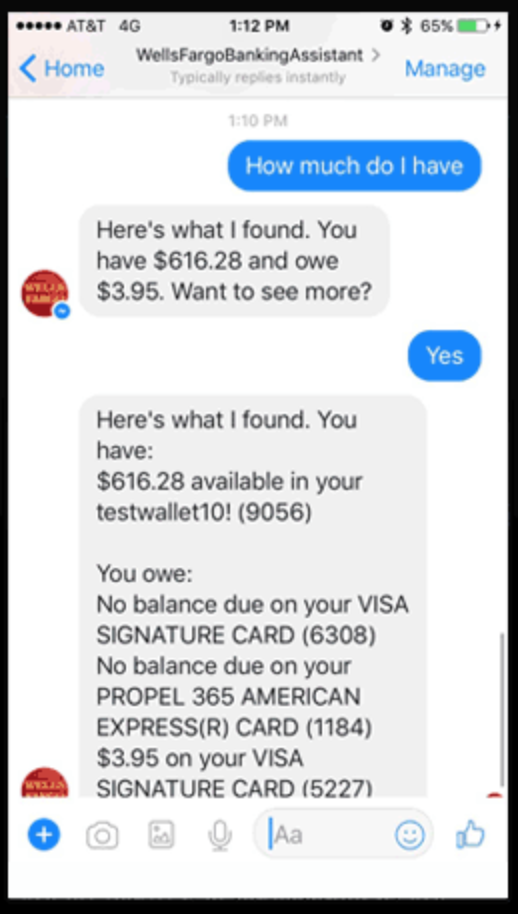
\includegraphics[width=0.3\textwidth, keepaspectratio]{images/wells_fargo_bot_1.png}
    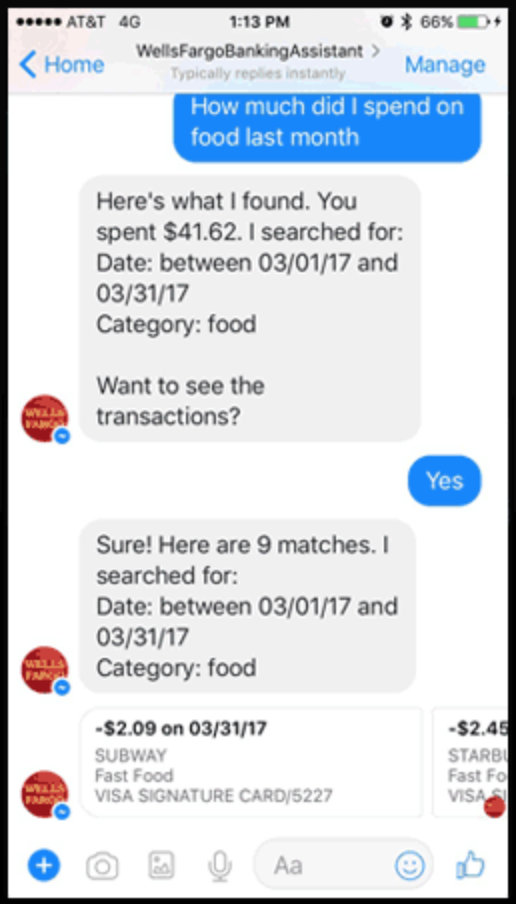
\includegraphics[width=0.3\textwidth, keepaspectratio]{images/wells_fargo_bot_2.png}
    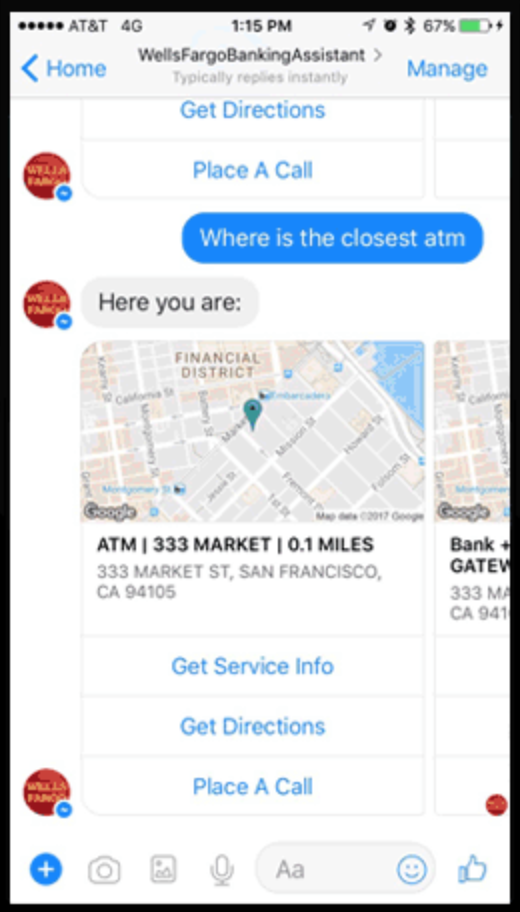
\includegraphics[width=0.3\textwidth, keepaspectratio]{images/wells_fargo_bot_3.png}
    \caption{Frontend of a Bank Assistant chat-bot by Wells Fargo on a Facebook}
    \medskip
    \footnotesize\textit{Source:} Own study
\end{figure}

Overwhelmingly, as a frontend, chatbots use textual dialog messenger and usually are associated with this form.
In this use-case customer write via suitable messenger, social network or application in an extremelly familiar environment.
Obviously, familiarity is also connected to prior existance of customer support dialogs in any form.
Nonetheless, as it was mentioned before, this is only a form of interaction, not a logic by itself and not the most labor-intensive part of the chatbot.


\subsection{Middleware}

Input received from frontend is passed to middleware.
Middleware can be either on a bank side, or on some third-party service.
Middleware is required for preprocesing of an input for processing on a bank side, or for postprocessing of an output received from a bank side for proper customer understanding.
In other words, this is a part of logic not connected to banking operations, but is required for proper understanding on both sides of interaction.

The most simple case is for Rule-based decision-making.
For this option there is no need to use complicated Statistics and Machine Learning knowledge, but input is represented by limited set of options and output is presented as a filled template answer.
This case is preferred for faster chat-bot development, or for a chat-bot on an employee side, which is hidden from a client. 

Nevertheless, middleware can have a much more complicated form.
Ideally, this is the first frontier of Artificial Intelligence and Machine Learning technics in chatbots
However, it is not used for analytics, but mainly for Natural Language Processing.

Natural Language Processing, NLP, divides in two parts — Natural Language Understanding and Natural Language Generation.
Natural Language Understanding is a branch of NLP which uses Artificial Intelligence, mostly Machine Learning technics, for building software to understand input in the form of sentences using text or speech.
Natural Language Generation is a branch of NLP which uses Artificial Intelligence, mostly Machine Learning technics, for building software to generate text and synthesize tet.

Accordingly, Conversational Banking has to be created with two instruments, Natural Language Understanding for input and Natural Language Generation for output.
Moreover, same middleware can be used for various forms, as a text or speech understanding framework for call-center bots, website chatbots or roboadvisers and for text or speech generation for SMS, text answers or cold calling.
 

\subsection{Backend}

Backend part of any conversational interaction is the most important from a banking side, as it is directly connected to banking processes.
This part is actual part of execution of transactions, request or for other orders of operations, including current balance check.
Moreover, it is inextricably linked with actual bank as a platform for financial services.
In comparison to frontend, interface for bank interaction has to be strictly formulated and defined, as, basically, this represents API, application programming interface, of a bank.

The most intense usage of AI is possible here and can be shared with all levels of banking.
The root source of data for decision-making based on AI is a metadata collected from requests.
As those request interface is strictly formulated, it is possible to define which type of data to collect, obviously, confirmed to GDPR regulations and requirements, and after proper anonymizing of corresponding data.
Backend of a chatbot should be connected to general recommendation system of a bank, as conversational banking, from a bank perspective, is yet another channel for client interaction.
Obviously, mentioned recommendation system is a main source of Machine Learning based decision-making, as it can build unpredictable models of client behaviour, both individual and as a group, and based on those models observe future client trends, give recommendations and what is even more important, contact with a client based on a made decision.

Secondly, this is a place for AI to learn customer related questions not connected to bank services, but to regulations.
For example, using supervised learning AI can learn, based on previous answers by a contact center, what documents client need to open current account or be informed about entire process of opening brokerage account.


\subsection{Conclusion}

Chatbots are an extremelly form of client interaction.
Even though latest achievements of Artificial Intelligence can and has to be applied to banking, those can be comparingly independent and developed separately and parallelly by different parties.
Moreover, those parts can be connected to existing banking services and interfaces and don't require changes other, than those required by modern banking regulations or Open Banking philosophy.
Banks can use same chatbot communication channel for notifications to increase level of client engagement.
In general, live chat can be used as a direct client communication channel with clients, provide information on product specs and services, contact info, payments proceeding, financial recommendations and many other goods and services.

It is possible to highlight several trends, which may have the most significant impact on the development of the chatbot industry in the near future.
Firstly, growth of share of combined solutions, in which robots are not able to replace human completely, but complement for repeating routine activities.
The most promising among of them are assistants for human operators, that are integrated with Robotic Process Automation.
The second trend is the development of tools for business intelligence data mining and building ontologies for unstructured data.
In other words, those are the systems into which it is possible to upload a variety of texts, and it will automatically
extract semantic connections and build language models, specific for that certain domain.
Lastly, shareable knowledge between different chatbots and chatbot platforms.
That would allow creating personified virtual assistants, with the special “personality” for each client.
As a result, we can say that Artificial Intelligence and Machine Learning mostly are being used by Front Office in a hidden for an ordinary man.
